%%%%%%%%%%%%%%%%%%%%%%%%%%%%%%%%%%%%%%%%%%%%%%%%%%%%%%%%%%%%%%%%%%%%%%%%%%%%%%%
% Chapter 2: Documented Design
%
% Required documentation for 'Documented Design'
% - The type of system that a student is developing will determine the aspects
%   of the system that need to be covered in documented design. It is anticipated
%   that for all systems, a high level overview of how different parts of the
%   system would interact would be usefull, this may be a:
%	- Structure / Heirarchy chart
%   - A system flowchart
%   - A data flow diagram, or object / class diagrams, accompanied by any further
%	  explaination that is helpful
%	- non-standard diagrams that combine elements of data flow and program
%	  control are accepted, as long as the two can be clearly distinguished
% - Students should also document how the important parts of their system work
%	Possible items that might be in design could be:
%	- Algorithms
%	- Data Structures
%	- File Structure and organisation
%	- Database design
%	- Queries
%	- Human Computer Interaction
%	- Hardware selection/design
%%%%%%%%%%%%%%%%%%%%%%%%%%%%%%%%%%%%%%%%%%%%%%%%%%%%%%%%%%%%%%%%%%%%%%%%%%%%%%%

\definecolor{listinggray}{gray}{0.9}
\definecolor{lbcolor}{rgb}{0.9,0.9,0.9}

\lstset{
backgroundcolor=\color{lbcolor},
    tabsize=4,    
%   rulecolor=,
    language=[GNU]C++,
    basicstyle=\scriptsize,
    upquote=true,
    aboveskip={1.5\baselineskip},
    columns=fixed,
    showstringspaces=false,
    extendedchars=false,
    breaklines=true,
    prebreak = \raisebox{0ex}[0ex][0ex]{\ensuremath{\hookleftarrow}},
    frame=single,
    numbers=left,
    showtabs=false,
    showspaces=false,
    showstringspaces=false,
    identifierstyle=\ttfamily,
    keywordstyle=\color[rgb]{0,0,1},
    commentstyle=\color[rgb]{0.026,0.112,0.095},
    stringstyle=\color[rgb]{0.627,0.126,0.941},
    numberstyle=\color[rgb]{0.205, 0.142, 0.73}}
\lstset{
    backgroundcolor=\color{lbcolor},
    tabsize=4,
    language=C++,
    captionpos=b,
    tabsize=3,
    frame=lines,
    numbers=left,
    numberstyle=\tiny,
    numbersep=5pt,
    breaklines=true,
    showstringspaces=false,
    basicstyle=\footnotesize,
%  identifierstyle=\color{magenta},
    keywordstyle=\color[rgb]{0,0,1},
    commentstyle=\color[rgb]{0,0.4,0},
    stringstyle=\color{red}}

\newpage
\chapter{Documented Design}

\section{High-Level Overview of System}

\section{Project Versioning}
\subsection{File Structure}

This section will talk about the general file structure I will be using and the style that I will be coding against. We will be using an example file, file_structure.cc, which is shown below.
    
\lstinputlisting[language=C++]{file_structure.cc} 

\subsubsection{File Header}

Firstly we will be looking at the generic file header for the \textit{.h} and \textit{.cc}  files used in my project. The file header is given below:

\lstinputlisting[language=C++, linerange={1-9}]{file_structure.cc}

There are 5 key sections included in the file header,
\begin{itemize}
\item{@file - this declared the name of the file, including its extension}
\item{@date - this is the date of creation of the file}
\item{@version - this documents what the version of the file is. It will change when there are small changes and when there are large changes. The significance of the change is shown by which number is changed, e.g. changing from version 0.01 to 0.1 is a more significant change than going from version 0.01 to 0.02}
\item{@brief - this is where a brief description of what the files purpose is and what it contains}
\item{@author - this is where the author of the files name is given}
\end{itemize}

The reason I am including a header block is because when browsing through my project most people will not be able to meticulously go through all the code working out what it does exactly. The header block serves for the purpose of explaining what the code in the file does, giving the reader any key information like version, date of creation and author as soon as they look at the file. This way the reader doesn't have to read all the code, they can just read the header block and they will understand, on a high level, what that section of the code does.  

\subsubsection{File Commenting}

Throughout the project I will be sticking to a particular commenting style, which applies rules to how document my code. This section explains how I comment and what style I use for each scenario.

The first area we will look at is how we document classes, their members and their methods. We will look at the example class B and in our file_structure.cc example file. The class extract is shown below.

\paragraph{Classes}

An extract of our example classes is given below:

\lstinputlisting[language=C++, linerange={12-31,53-55}]{file_structure.cc}

A class will contain 4 sections:
\begin{itemize}
\item{@class - The name of the class, the name should also always use CamelCasing}
\item{@version - The current version of the class}
\item{@implements - If the class inherits from another class then the name of the inherited class is given here}
\item{@brief - This provides a short explanation of what the class does and what its purpose is}
\end{itemize}

\paragraph{Methods}

An extract of class method documentation is given below:

\lstinputlisting[language=C++, linerange={30-49,55}]{file_structure.cc}

\begin{itemize}
\item{@brief - Explains what the method does}
\item{@param - If the method takes parameters then these will be declared and explained here}
\item{@return - If the method returns something this explains what that is}
\item{Then after these tags a more detailed explanation of what happens in the method will be given below}
\end{itemize}

\paragraph{Members}

An extract of class member documentation is given below

\lstinputlisting[language=C++, linerange={30-31,51-55}]{file_structure.cc}

\begin{itemize}
\item{Next to the member use the style {\color{green} \textit{/**$<$  */} } to describe what its purpose in the class is}
\end{itemize}

\subsection{Version Changelog}

Lets look at the file header again, it is given below:

\lstinputlisting[language=C++, linerange={1-9}]{file_structure.cc}

As you can see there is a {\color{green} \textit{@version}} tag. For every data structure and file in the project there will the a  {\color{green} \textit{@version}} tag which will contain the most up to date version of the file / data structure. This allows me to easily keep track of how each element of my project is progressing and evolving. The behavior of this tag is explained in \textit{Section 2.2.1.1}. 




\subsection{Off-Site Backups}

When developing a project of this scale it is crucial that you don't just \textit{keep all your eggs in one basket} per say. What I mean by this is that you don't want a single point of failure, if I finished my project and then a week before the submission date my laptop died and I couldn't recover the data from my hard-drive then I would not be able to submit my project and I would fail.

For this reason I will be using Github to store daily backups of my projects code and documentation. This way, even if my laptop dies and I have no way of recovering the data I would have only lost a days worth of work, rather than a few months of work. 

This will not actually affect the end result of my project but I do feel it is important to talk about it as it is probably the most important step of all since if something goes wrong, you can recover, if you don't you cant. 

\section{Bespoke Algorithm Design}

\section{Cryptographic Algorithm Design}

\subsection{Galois Fields for AES}

In AES, every single operation that is used is based on Finite Fields. This section will give you a brief introduction to what Finite Fields are and how they are used.

\subsubsection{Introduction to Finite Fields}

It should be stated now that the term \textit{Finite Field} means the same thing as the term \textit{Galois Field}. In Abstract Algebra there are 3 basic structures, the group, the ring, and the finite field.

\paragraph{Groups Definition}
A group is a set of elements $G$ together with an operation $\cdot$ which contains $2$ elements of $G$. A group has the following properties:
\begin{enumerate}
\item{The group operator $\cdot$ is closed. That is for all $a,b \in G$, it holds that $a \cdot b = c \in G$}
\item{The group operation is associative. That is, $a \cdot (b \cdot c) \equiv (a \cdot b) \cdot c$ for all $a,b,c \in G$}
\item{There is an identity element $1 \in G$ such that $a \cdot 1 = 1 \cdot a = a$ for $a \in G$}
\item{There is an inverse element for all elements in $G$. That is for $a \in G$, there must be a element $a^{-1} \in G$ such that $a \cdot a^{-1} = a^{-1} \cdot a = 1$}
\item{A group is Abelian (or commutative) if, $a,b \in G$, $a \cdot b \equiv b \cdot a$}
\end{enumerate}

Roughly speaking a group is set with one operation and its corresponding inverse operation. If this operation is addition then the inverse operation will be subtraction, if the operation is multiplication then the inverse will be division. If we need a structure that can hold all 4 operations, that is where we will use Finite Fields (Galois Fields). It should be noted that it is common to denote a Finite Field as FF and a Galois Field as GF. 

\paragraph{Finite Field Definition}

A field $F$ is a set of elements with the following properties:

\begin{enumerate}
\item{All elements of $F$ for an additive group with the group operation "$+$" and the identity element $0$.}
\item{All elements of $F$, except the identity element $0$, form a multiplicative group with the group operation "$\times$" and the identity element $1$.}
\item{When the two group operations are mixed, the distributivity law holds, e.g. for all $a,b,c \in F : a(b + c) = (ab) + (ac)$} 
\end{enumerate}

In cryptography we are almost always interested in fields with a finite number of elements which we intuitively name Finite Fields or Galois fields. The number of elements in the field is called the \textit{order} or \textit{cardinality} of the field. It should be noted that a field with order $m$ only exists if $m$ is a prime power, e.g. $m = p^n$ where $n$ is a positive integer and $p$ is a prime number. $p$ is called the characteristic of the finite field. This implies that there are finite fields with $11$ elements or $81$ elements, since $81 = 3^4$ or with 256 elements (since $256 = 2^8$ and $2$ is a prime). There is no finite fields with 12 elements since $12 = 2^2 \cdot 3$ and 12, meaning 12 is not a prime power.

\paragraph{Prime Fields}

The most intuitive examples of FF are fields of prime order, fields with $n=1$. Elements of the $GF(p)$ can be represented by the integers $0,1,...,p-1$. The two operations are modular integer addition and multiplication modulo $p$. This means that if we consider the integer ring $\mathbb{Z}_m$ and $m$ happens to be prime then $\mathbb{Z}_m$ is not only a ring but also a finite field.

In order to do arithmetic in a prime field we have to follow the rules for integer rings:  Addition and multiplication are done modulo $p$, the additive inverse of any element $a$ is given by $a + (-a) = 0 \bmod p$, and the multiplicative inverse of any non-zero element $a$ is defined as $a \cdot a^{-1} = 1$ 

We can look at the example of the prime field $GF(2) = \{0,1\}$, which is the smallest finite field that can exist. The additive and multiplicative tables for the GF are listed below.


\begin{table}[h!]
\begin{center}
\begin{tabular}{ |c|cc| } 
 \hline
 + & 0 & 1 \\ 
 \hline
 0 & 0 & 1 \\ 
 1 & 1 & 0 \\ 
 \hline
\end{tabular}
\caption{Additive Table for $GF(2)$}
\label{GF-2-Addition}
\end{center}
\end{table}

\begin{table}[h!]
\begin{center}
\begin{tabular}{ |c|cc| } 
 \hline
 $\times$ & 0 & 1 \\ 
 \hline
 0 & 0 & 0 \\ 
 1 & 0 & 1 \\ 
 \hline
\end{tabular}
\caption{Multiplicative Table for $GF(2)$}
\label{GF-2-Multiplicative}
\end{center}
\end{table}

This is quite cool as it shows that addition in $GF(2)$, modulo 2 addition, is equivalent to and XOR Gate. It also shows us that multiplication in $GF(2)$ is equivalent to the logical AND Gate. This field, $GF(2)$ is very important for AES.

\subsubsection{Extention Fields $GF(2^m)$}  

AES uses a FF of 256 elements and is denoted as $GF(2^8)$. This field was chosen as each of the elements in this field can be represented as exactly one byte. It becomes increasing important as the S-Box and MixColumn transformations treat every byte of the internal data path as an element of the field $GF(2^8)$ and manipulates the data by performing arithmetic in this finite field.

As we said before if the order of a FF is not prime, which is clearly the case here ($2^8$ is clearly not a prime number) the addition and multiplication operators can not be represented by addition and multiplication of integers modulo $2^8$. Fields with $m>1$ are called \textit{extension fields}. In order for us to have the ability of working with these fields we need the following:

\begin{enumerate}
\item{A different notation for the field elements}
\item{Different rules for when we perform arithmetic operations with the elements}
\end{enumerate}

So for the elements of these finite fields, we represent them as \textit{polynomials} with coefficients and that when we compute with these we perform a certain type of \textit{polynomial arithmetic}. The polynomials have a maximum degree of $m-1$, so that there are $m$ coefficients in total for every element. In the field $GF(2^8)$, which is the AES FF, each element $A \in GF(2^8)$ is represented as:

\begin{center}
$A(x) = a_7x^7 + a_6x^6 + ... + a_1x + a_0$ where \\
$a_i \in GF(2) = \{0,1\}$
\end{center}

It is very important to realise that every element of $GF(2^8)$ can also be stored as an $8-bit$ vector:

\begin{center}
$A = (a_7,a_6,a_5,a_4,a_3,a_2,a_1,a_0)$
\end{center}

This means we do not have to store the factors $x^7,x^5,etc$ as it is clear from the bit positions to which power $x^i$ each coefficients belongs.

\subsubsection{Addition and Subtraction in $GF(2^m)$}

This is actually really easy as we just follow the basic polynomial rules of addition and subtraction, we just add or subtract coefficients with equal powers of $x$. This is mathematically shown below, Let $A(x), B(x) \in GF(2^m)$. The sum of the two elements is then computed as the following: 

\begin{center}
$$C(x) = A(x) + B(x) = \sum_{i=1}^{m-1} c_ix^i$$ where
$c_i \equiv a_i + b_i \bmod 2$
\end{center}

and the difference between the 2 pairs is computed as the following:

\begin{center}
$$C(x) = A(x) - B(x) = \sum_{i=1}^{m-1} c_ix^i$$ where
$c_i \equiv a_i - b_i \equiv a_i + b_i \bmod 2$
\end{center}

Since we perform modulo 2 addition with the coefficients, addition and subtraction are the same thing. An example of this is given below:

\begin{center}
\begin{align*}
A(x) &= x^7 + x^6 + x^4  + 1 \\
B(x) &= x^4 + x^2 + 1 \\
C(x) &= A(x) + B(x) = x^7 + x^6 + x^2
\end{align*}
\end{center}

Note if we were to work out the difference between the two polynomials $A(x)$ and $B(x)$ it would be the same as $C(x)$.

\subsubsection{Multiplication in $GF(2^m)$}

Multiplication in $GF(2^8)$ is the core operation in the MixColumn transformation in AES. Firstly, 2 elements of $GF(2^8)$ are multiplied using standard polynomial rules:

\begin{center}
\begin{align*}
A(x) \cdot B(x) &= (a_{m-1}x^{m-1} + ... + a_0) \cdot (b_{m-1}x^{-1} + ... + b_0) \\
C\textprime(x) &= c\textprime_{2m-2}x^{2m-1} + ... + c\textprime_0
\end{align*}

Where:

\begin{align*}
c\textprime_0 &= a_0b_0 \bmod 2 \\
c\textprime_1 &= a_0b_1 + a_1b_0 \bmod 2 \\
&. \\
&. \\
&. \\
c\textprime_{2m-2} &= a_{m-1}b_{m-1} \bmod 2
\end{align*}

\end{center}

Realize that all coefficients $a_i$, $b_i$ and $c_i$ are elements of $GF(2)$ and that coefficients arithmetic is performed in $GF(2)$. In general the product polynomial, $C(x)$, will have a degree higher than $m-1$ and will thus have to be reduced. The idea is similar to what we would do in prime fields: in $GF(p)$, we multiply  the two integers, divide the result by a prime and consider only the remainder. In extension fields the product polynomial $C(x)$ is divided by a special polynomial and we consider only the remainder after the polynomial division. The special polynomials are called irreducible polynomials and we need them for the module reduction. These polynomials are roughly comparable to prime numbers, basically their only factors are 1 and the polynomial itself. A mathematical description of Extension Field multiplication is given below:

Let $A(x), B(x) \in GF(2^m)$ and let 

\begin{center}
$$ P(x) \equiv \sum_{i=0}^{m} p_ix^i, p_i \in GF(2) $$
\end{center}

be an irreducible polynomial. Multiplication of the two elements $A(x), B(x)$ is given as

\begin{center}
$C(x) \equiv A(x) \cdot B(x) \bmod P(x)$
\end{center}

This means that we need a irreducible polynomial $P(x)$, of degree $m$ and with coefficients from $GF(2)$, for every field $GF(2^m)$. Not all polynomials are reducible much like not every number is a prime. We only need to know the irreducible polynomial for AES; it is given below

\begin{center}
$P(x) = x^8 + x^4 + x^3 + x + 1$
\end{center}

This polynomial is a part of the specification for AES. 

Putting this all together, lets say that we have the 2 polynomials $A(x)$ and $B(x)$ where $A(x) = x^3 + x^2 + 1$ and $B(x) = x^2 + x$ and we want to multiply them in the $GF(2^4)$. The irreducible polynomial for this GF is given as $P(x) = x^4 + x + 1$.

First we have to work out the plain polynomial multiplication,

\begin{center}
$C\textprime(x) = A(x) \cdot B(x) = x^5 + x^3 + x^2 + x $
\end{center}

We can now reduce $C\textprime(x)$ using the standard polynomial division method, but it can sometimes be easier to reduce each of the leading terms $x^4$ and $x^5$ individually.

\begin{center}
\begin{align*}
x^4 &= 1 \cdot P(x) + (x+1)\\
x^4 &\equiv x + 1 \bmod P(x) \\
x^5 &\equiv x^2 + x \bmod P(x)
\end{align*}
\end{center} 

Now we just substitute that back into our $C\textprime(x)$ expression and we will get our result for the multiplication of $A(x)$ and $B(x)$

\begin{center}
\begin{align*}
C(x) &\equiv x^5 + x^3 + x^2 + x \bmod P(x) \\
C(x) &\equiv (x^2 + x) + (x^3 + x^2 + x) = X63 \\
A(x) \cdot B(x) &\equiv x^3 \\
\end{align*}
\end{center}

We need to make sure we do not confuse multiplication in $GF(2^m)$ with integer multiplication, especially if we are concerned with software implementations of Galois fields.

\subsubsection{Inversion in $GF(2^m)$}

Inversion in $GF(2^8)$ is the core operation in the Byte Substitution Layer of AES which contains the S-Boxes. For a given FF $GF(2^m)$ and the corresponding irreducible polynomial $P(x)$, the inverse $A^{-1}$ of a nonzero element $A \in GF(2^m)$ is defined as:

\begin{center}
$A^{-1} \cdot A(x) = 1 \bmod P(x)$
\end{center}

For small fields, in practice fields with $2^16$ or fewer elements, look-up tables which contain the precomputed inverses of all finite elements are often used. Figure \ref{AES-RS-BOX} shows the multiplicative inverse for $GF(2^8)$ used in AES.

\begin{figure}[h!]
\begin{center}
\includegraphics[scale=1]{aes-rsbox.png}
\caption{The multiplicative inverse table of $GF(2^8)$ for bytes $xy$ used within the AES S-Box}
\label{AES-RS-BOX}
\end{center}
\end{figure}

As an alternative to using lookup tables, it is possible to compute the inverses of all the elements. The main algorithm uses for this task is the Extended Euclidean Algorithm (EEA).

\subsection{AES Internals}
\subsubsection{Structure of AES}

It should be noted that the 128-bit data path that runs through the algorithm is split up into 16-bytes, this is why many people would consider AES a byte oriented block cipher as it works in pure bytes. So our structure diagram from Figure \ref{AES-HL-Overview} can be adapted to the structure shown in Figure \ref{AES-BL-Overview}. We also noted before that the algorithm operates on a $4\times4$ matrix of bytes, Figure \ref{AES-Byte-Ordering}, and this remains true so keep that in mind when performing any operations, this becomes especially important in the ShiftRows and MixColumns steps.

\begin{figure}[h!]
\begin{center}
\includegraphics[scale=0.5]{aes-bl-overview-ue.png}
\end{center}
\caption{AES Byte Level Overview}
\label{AES-BL-Overview}
\end{figure}

The rest of this section will be looking into how the different components of each round work, these being the ByteSub Layer, ShiftRows Layer, MixColumns Layer and Key Addition Layer.

\subsubsection{Byte Substitution Layer}

The first layer in AES is the Byte Substitution Layer. There are 16 parallel S-Box which all take 8-bits as input and 8-bits as output. All 16 S-Box are identical with is different to DES as that cipher uses 8 unique S-Boxes. Each state Byte $A_i$ is replaced, substituted, with another Byte, $B_i$. The process is shown below:

\begin{center}
$S(A_i) = B_i$
\end{center}

The S-Box is the only non-linear section of AES. This basically means that

\begin{center}
$S(A) + S(B) \neq S(A + B)$
With 2 Byte States $A$ and $B$.
\end{center}

The S-Box substitution is a 1-to-1 mapping, basically all of the $2^8 = 256$ elements are mapped to one output element. This is good as it allows us to uniquely reverse the S-Box, which is key to the decryption process. In software, the S-Box is usually setup as a 256 Byte lookup table with fixed entries. The AES S-Box is given below for an input byte $(YX)$, with $(YX$) representing its hexadecimal value in each of its respective columns.

\begin{figure}[h!]
\begin{center}
\includegraphics[scale=0.7]{aes-sbox.png}
\end{center}
\caption{The AES S-Box}
\label{AES-S-BOX}
\end{figure}

So lets look at an example, say we have the Byte State $A_i = (3b)_{hex}$, then we apply the S-Box and get the following result:

\begin{center}
$S(A_i) \equiv S((3b)_{hex}) \equiv (e2)_{hex}$
\end{center}

If we were to look at this on a bit level, the point of interest for the cryptography of the cipher, then the substitution becomes:

\begin{center}
$S(A_i) \equiv S(00111011) \equiv (11100010)$
\end{center}

Even though the S-Box has a 1-to-1 mapping, it does not have any fixed points. This means that there are no input values $A_i$ that make $S(A_i) = A_i$. Even the zero-input state is not a fixed point, i.e $S((00)_{hex}) = S(00000000) = (01100011)$.

\paragraph{Mathematical Description of S-Box}

\begin{center}
ADD THIS IN LATER
\end{center}

\subsubsection{ShiftRows Layer}

The ShiftRows Layer does exactly what its name implies. It cyclically shifts the rows of the byte matrix, see Figure \ref{AES-Byte-Ordering}. It shifts the first row by 0 bytes, the second row by 1 byte to the left, the third row 2 bytes to the left and the fourth row by 3 bytes to the left. If we take out original byte matrix, also shown in Figure \ref{AES-Byte-Ordering}, shown below:

\begin{center}
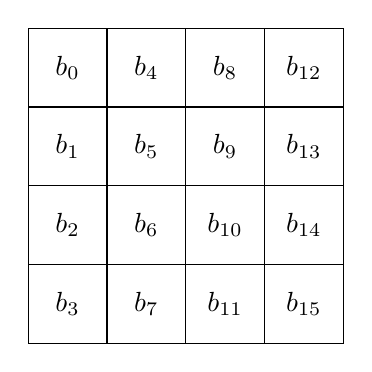
\begin{tikzpicture}[scale=1]

	\draw (0,3) rectangle node { $b_0$} +(1,1);
	\draw (0,2) rectangle node { $b_1$} +(1,1);
	\draw (0,1) rectangle node { $b_2$} +(1,1);
	\draw (0,0) rectangle node { $b_3$} +(1,1);
	\draw (1,3) rectangle node { $b_4$} +(1,1);
	\draw (1,2) rectangle node { $b_5$} +(1,1);
	\draw (1,1) rectangle node { $b_6$} +(1,1);
	\draw (1,0) rectangle node { $b_7$} +(1,1);
	\draw (2,3) rectangle node { $b_8$} +(1,1);
	\draw (2,2) rectangle node { $b_9$} +(1,1);
	\draw (2,1) rectangle node { $b_{10}$} +(1,1);
	\draw (2,0) rectangle node { $b_{11}$} +(1,1);
	\draw (3,3) rectangle node { $b_{12}$} +(1,1);
	\draw (3,2) rectangle node { $b_{13}$} +(1,1);
	\draw (3,1) rectangle node { $b_{14}$} +(1,1);
	\draw (3,0) rectangle node { $b_{15}$} +(1,1);
        
\end{tikzpicture}
\end{center}

After the ShiftRows Layer, the matrix would look like this, shown below.

\begin{center}
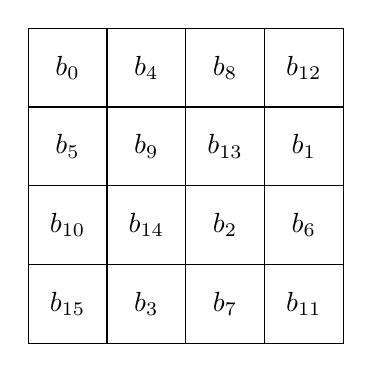
\begin{tikzpicture}[scale=1]

	\draw (0,3) rectangle node { $b_0$} +(1,1);
	\draw (0,2) rectangle node { $b_5$} +(1,1);
	\draw (0,1) rectangle node { $b_{10}$} +(1,1);
	\draw (0,0) rectangle node { $b_{15}$} +(1,1);
	\draw (1,3) rectangle node { $b_4$} +(1,1);
	\draw (1,2) rectangle node { $b_9$} +(1,1);
	\draw (1,1) rectangle node { $b_{14}$} +(1,1);
	\draw (1,0) rectangle node { $b_3$} +(1,1);
	\draw (2,3) rectangle node { $b_8$} +(1,1);
	\draw (2,2) rectangle node { $b_{13}$} +(1,1);
	\draw (2,1) rectangle node { $b_{2}$} +(1,1);
	\draw (2,0) rectangle node { $b_{7}$} +(1,1);
	\draw (3,3) rectangle node { $b_{12}$} +(1,1);
	\draw (3,2) rectangle node { $b_{1}$} +(1,1);
	\draw (3,1) rectangle node { $b_{6}$} +(1,1);
	\draw (3,0) rectangle node { $b_{11}$} +(1,1);
        
\end{tikzpicture}
\end{center}

\subsubsection{MixColumns Layer}

The MixColumns Layer is a linear transformation step which mixes the column of the state matrix. The combination of the ShiftRow and MixColumn layers makes it possible that after only three rounds, every byte of the state matrix depends on all 16 plaintext bytes. We denote the MixColumn layer with input matrix B and output matrix C as the following:

\begin{center}
MixColumn(B) = C
\end{center}

Where B is the state matrix after the ShiftRows layer. Now we take each column as a vector and is then mulitplied by a fixed $4 \times 4$ matrix. This matrix is constant. Multiplication and addition of the coefficients is done in $GF(2^8)$. The computation of the first four output bytes is shown below.
\begin{center}
$
\begin{pmatrix}
C_0 \\
C_1 \\
C_2 \\
C_3
\end{pmatrix} 
$
=
$
\begin{pmatrix}
02 & 03 & 01 & 01 \\
01 & 02 & 03 & 01 \\
01 & 01 & 02 & 03 \\
03 & 01 & 01 & 02
\end{pmatrix}
$
$
\begin{pmatrix}
B_0 \\
B_5 \\
B_{10} \\
B_{15} 
\end{pmatrix}
$
\end{center}

The second column of C, $(C_4, C_5, C_6, C_7)$ is computed by multiplying the same constant matrix by $(B_4, B_9, B_{14}, B_3)$, the third and fourth columns of C ad heed to this as well. 

We know that each state byte, $C_i$ and $B_i$ are 8-bit values that represent a value in $GF(2^8)$. All arithmetic done is performed in this layer is formed in $GF(2^8)$. The constants in the matrix are hexadecimal numbers, representing the corresponding values in the Galois Field. So $01_{hex}$ is $00000001_{bin}$ which corresponds to the $GF(2^8)$ element 1, $02_{hex}$ is $00000010_{bin}$ corresponds to the $GF(2^8)$ polynomial $x$ and $03_{hex}$ is $00000011_{bin}$ corresponds to the $GF(2^8)$ polynomial $x+1$. 

The additions here are performed in $GF(2^8)$ so are simple XOR operations with the 2 different bytes. For the multiplications, the constants $01,02,03$ were chosen as they are very easy to set up in software. Multiplication with $01$ is just multiplication by the identity which doesn't require a given operation. Multiplication by $02$ and $03$ are more complicated, therefore 2 $256$ byte lookup tables are used. You could do multiplication by $02$ as a multiplication by $x$, which is just a left shift of 1, and then a modular reduction by the irreducible polynomial of $GF(2^8)$, $P(x) = x^8 + x^4 + x^3 + x + 1$. Multiplication by $03$ is similar, it is just a left shift of 1 and then adding the original value followed by modular reduction of $P(x)$ again.

As an example, lets take the input state array, $B = (25,25,...,25)$. Since we are only doing the first column this only involves 2 multiplications, by $02$ and $03$. 

\vspace{-1cm}
\begin{center}
\begin{align*}
02 \cdot 25 =& \hspace{0.3cm} x \cdot (x^5 + x^2 + 1) \\
            =& \hspace{0.3cm} x^6 + x^3 + x \\
03 \cdot 25 =& \hspace{0.3cm} (x + 1) \cdot (x^5 + x^2 + 1) \\
            =& \hspace{0.3cm} (x^6 + x^3 + x) + (x^5 + x^2 + 1 \\
            =& \hspace{0.3cm} x^6 + x^5 + x^3 + x^2 + x + 1
\end{align*}
\end{center}

Since the order of our intermediate values, $x^6 + x^3 + x$ and $x^6 + x^5 + x^3 + x^2 + x + 1$, do not have an order of above $8$ we don't need to perform modular reduction with $P(x)$, the next step is to add together all the components of the multiplication.

\vspace{-1cm}
\begin{center}
\begin{align*}
02 \cdot 25 &= \hspace{0.3cm} 1x^6 + 0x^5 + 0x^4 + 1x^3 + 0x^2 + 1x + 0 \\
03 \cdot 25 &= \hspace{0.3cm} 1x^6 + 1x^5 + 0x^4 + 1x^3 + 1x^2 + 1x + 1 \\
01 \cdot 25 &= \hspace{0.3cm} 0x^6 + 1x^5 + 0x^4 + 0x^3 + 1x^2 + 0x + 1 \\
01 \cdot 25 &= \hspace{0.3cm} 0x^6 + 1x^5 + 0x^4 + 0x^3 + 1x^2 + 0x + 1 \\
\cline{1-2} \\
C_i &= \hspace{0.3cm} 0x^6 + 1x^5 + 0x^4 + 0x^3 + 1x^2 + 0x + 1
\end{align*}
\end{center}

This is where $i = 0,1,2,...,15$. This means our output state is the value of the $GF(2^8)$ polynomial $x^5 + x^2 + 1$ which is $25$. So $C = (25,25,...,25)$. 
 
\subsubsection{Key Addition Layer}

The key addition layer takes 2 inputs, the current 16-byte state matrix and a sub key which is also 16-bytes. Then the 2 inputs are combined using the XOR operation. The particular sub keys that are derived are explained in the next section, \textit{Section 2.4.2.6}.

\subsubsection{AES Key Schedule}

The Key Schedule takes our original 128/192/256 bit key and will then derive the subkeys needed for the algorithm. At the beginning and end of AES a XOR addition is applied to the subkey, this process is sometimes referred to as key-whitening. The number of subkeys required is the number of rounds plus one as we need an extra subkey for the key-whitening. A table with the key lengths, round numbers, and subkeys is shown below.

\begin{table}[h!]
\begin{center}
\begin{tabular}{ c|c|c } 
$N_k (bits)$ & $N_r$ & $N_{sk}$ \\
\hline
$128$ & $10$ & $11$ \\
$192$ & $12$ & $13$ \\
$256$ & $14$ & $15$ \\
\end{tabular}
\caption{Repsective Key Lengths, Rounds Numbers, Subkey Numbers}
\label{AES-KeyL-RoundNumber-Subkeys}
\end{center}
\end{table}

The AES Key Schedule is word oriented, where 1 word $=$ 32-bits. Sub keys are stored in an expansion array called $W$ that consists of words. There are 3 different key schedules for the 3 different key sizes.

\paragraph{128-bit Key Schedule}
\paragraph{192-bit Key Schedule}
\paragraph{256-bit Key Schedule}

\subsection{Decryption in AES}

\subsubsection{Inverse MixColumns Layer}

\subsubsection{Inverse ShiftRows Layer}

\subsubsection{Inverse ByteSubstitution Layer}

\subsubsection{Decryption Key Schedule}



\subsection{DES}
\subsubsection{Structure of DES}
\subsubsection{Internals of DES}
\subsubsection{Operations with DES}

\section{Bespoke Data Structures}

\section{Bespoke Database Design}
\subsection{User Details}
a
\subsection{User Answers}
a
\subsection{Authentication Information}
a
\subsection{Authentication Identity}
a
\subsection{Authentication Token}
a
\subsection{Question Details}
a

\section{User Interface Design}
a
\subsection{Header}
a
\subsection{Information Window}
a
\subsection{Login Page}
a
\subsection{Register Page}
a

\section{System Security}
\subsection{Security Requirements}
\subsection{User Details Storage}

\section{External Library's}
\subsection{Wt}

Wt, said \textit{Witty}, is a Web framework for the C++ programming language. It provides the basic widgets and building blocks needed to create A Web Application but also has a lot of other really useful features. This include but are not limited to:

\begin{itemize}
\item{Client Side Optimized

By using a signal-slot system, we don't have to worry about dealing with the AJAX requests. We simply connect a widget to the callback function of the server and its done. It also will use whatever technology is available for use in the communication, normally AJAX or WebSockets, but if will fall back into full html page reloads if javascript is not available. This allows a Wt Application to be accessible to any browser}
\item{Built-In Security

By default, Wt only allows the visible and enable widgets to be interacted with. It also helps prevent CSRF attacks by not storing any of the session information in cookies. Because of the Widget abstraction it discourages the use of raw html in the application which helps to prevent again XSS attacks. SQL Injection attacks are stopped by encouraging the user to use prepared SQL statements when accessing the database. Wt also includes an authentication and registration system with support for OAuth providers like Google and Facebook}
\item{Object Relational Mapping Library

This maps C++ classes to tables in my database using Wt::Dbo, a ORM that only requires pure C++. It does not depend on preprocessor magic or code generation.}
\end{itemize}

\subsection{Crypto++}

Crypto++ is a C++ library that contains implementations for a huge amount of Cryptographic algorithms.

%For an investigative project; a log of stages taken during the investigation and how this affected the coding
